\documentclass[a4paper]{scrbook}

\usepackage[utf8]{inputenc}
\usepackage{listings}
\usepackage{graphicx}
\usepackage{booktabs}
\usepackage{url}
\usepackage{relsize}
\usepackage{hyperref}
\usepackage{tgtermes}
\usepackage{ifthen}
\usepackage{fancyhdr}
\usepackage{multirow}
\usepackage{verbatim}
\usepackage{color}

\lstset{frame=tb,
  language=c++,
  aboveskip=5mm,
  belowskip=5mm,
  showstringspaces=false,
  columns=flexible,
  basicstyle={\small\ttfamily},
  numbers=none,
  numberstyle=\tiny\color{blue},
  keywordstyle=\color{red},
  commentstyle=\color{pink}\string,
  stringstyle=\color{green},
  breaklines=true,
  breakatwhitespace=true,
  tabsize=4}
%%%%%%%%%%%%%%%%%%%%%%%%%%%%%%%%%%%%%%%%%%%%%%%%%%%%%%%%%%%%%%%%%%%%%%%%%%%%%%%%
% Replace these values
%%%%%%%%%%%%%%%%%%%%%%%%%%%%%%%%%%%%%%%%%%%%%%%%%%%%%%%%%%%%%%%%%%%%%%%%%%%%%%%%
\newcommand{\thesistitleDE}{Linux-Kernel-Treiber\\I2C Sensor und OLED Display}
\newcommand{\thesistitleEN}{Linux Kernel Driver\\I2C Sensor and OLED Display}
\newcommand{\student}{Nik Amir Syazwan Bin Abdul Aziz}
\newcommand{\matrnr}{00819429}
\newcommand{\stammnr}{00819429}
\newcommand{\submissiondate}{02.\ Juli 2023}
\newcommand{\supervisor}{Herr Tobias Gent}
\newcommand{\secsupervisor}{Herr Sergej Lamert}
\newcommand{\faculty}{Angewandte Informatik}

\newcommand{\studies}{Bachelor Angewandte Informatik}

\newcommand{\degree}{Bachelor of Engineering (B.Eng.)}

\renewcommand*{\UrlFont}{\ttfamily\smaller\relax}

\begin{document}
\pagestyle{headings}
\pagenumbering{roman}
\setkomafont{title}{\huge \scshape}
\begin{titlepage}
\begin{center}
	{\usekomafont{subject}
	Technische Hochschule Deggendorf\\
	Fakultät \faculty\par}
	\vspace{.2cm}
{\Large Studiengang \studies\\}
\vspace{6\baselineskip}
{\Huge\usekomafont{title}\thesistitleDE\par}
\vspace{1cm}
{\Huge\usekomafont{title}\thesistitleEN\par}
\vspace{6\baselineskip}

\usekomafont{publishers}
Bacheloarbeit zur Erlangung des akademischen Grades:

	\vspace{.2cm}
	\emph{\degree}
	\vspace{.2cm}

an der Technischen Hochschule Deggendorf\\
\end{center}
\vfill
\parbox[t]{.4\textwidth}{\usekomafont{author}
	Vorgelegt von:\\
	\student\\
	Matrikelnummer: \matrnr\par
	\ifthenelse{\equal{\stammnr}{}}{}
	\vspace{\baselineskip}
	Am: \submissiondate\par
}
\hfill
\parbox[t]{.4\textwidth}{\usekomafont{author}
Prüfungsleitung:\\
\supervisor%

\ifthenelse{\equal{\secsupervisor}{}}{}
{%
\vspace{\baselineskip}
Ergänzende Prüfende:\\
\secsupervisor%
}}
\end{titlepage}
\cleardoublepage\par


\chapter*{Abstract}
\addcontentsline{toc}{chapter}{Abstract}
As the usage of Linux becoming more popular in recent years, the development of linux drivers has improved significantly to
help and ease the users around the world. These drivers can be as simple as hardware driver for basic computer device
such as mouse, keyboard to much more complicated devices such as microprocessor and microcontroller for developers. The present 
report aims to outline the design, development, and implementation of a Linux kernel driver for I2C (Inter-Integrated Circuit) sensors 

The report begins by providing an overview of I2C communication and its significance in connecting various devices, especially 
sensors, to a Linux-based system. The characteristics and advantages of I2C bus architecture are discussed, emphasizing its 
suitability for sensor applications. The subsequent sections delve into the methodology employed for designing and implementing 
the Linux kernel driver for I2C sensors. The driver development process involves understanding the hardware specifications of the target sensor, 
defining necessary data structures and functions, and integrating them into the Linux kernel source code.

Additionally, the report discusses the challenges encountered during the driver development process, including data type problem, time management issues and 
lack of experience issue. The solutions and workarounds implemented to overcome these challenges are presented, 
highlighting the critical thinking and problem-solving skills employed.

In conclusion, the development and implementation of a Linux kernel driver for I2C sensors presented in this report provide a solid foundation 
for seamless integration and efficient utilization of I2C sensors within Linux-based systems.


\tableofcontents

\cleardoublepage%
\setcounter{page}{1}
\pagenumbering{arabic}
\chapter{Introduction}
Throughout the years the Linux system has gained massive attention do to its feature as a developer-friendly operating system and how accessible it is. And because of that, the rate of development of Linux device drivers has increased significantly allowing its users to configure their working environment more efficiently and ease the usage of Linux. Linux has now become a the go-to OS for most hardware including Raspberry Pi, which has its Operating System working under Linux. This documentation will provide the full details about the project of making Linux Kernel driver for an I2c sensor and OLED Display using Raspberry Pi.

\section{Overview}
Usually virtual memory is segregated into user space and kernel space in modern computer operating system. To handle communication from user space and kernel, a device driver is needed. A device driver is a piece of software interface to allow operating system or any software called user space applications to access and communicate with the hardware without any prior information about the hardware. A user space application is in the other hand, a software in the user space that uses this device driver to communicate with the hardware.The layers of communication between user application can be displayed as following figure Table~\ref{tab:table1}.

In this project, this mentioned hardware are an OLED Display SH1107 and an I2C temperature sensor TMP102. Linux distinguish three types of device which are character devices, block devices and network interfaces. The mentioned hardware are in the category of character devices and therefore classifiable as a char module. This character devices will usually implements open, close, read and write system calls \cite{rubini_linux_2001}
. In this category, there are slow devices, which manage a small amount of data, and access to data does not require frequent seek queries. Examples are devices such as keyboard, mouse, serial ports, sound card, joystick. In general, operations with these devices (read, write) are performed sequentially byte by byte \url{https://linux-kernel-labs.github.io/refs/heads/master/labs/device_drivers.html}. \\


\section{Purpose}
This purpose of this document is to provide the project report and as a documentation for the software created, especially of its usage. It will also provide simple information on how the hardware works with the software as further information can be read from the data sheets instead. The purpose of the project is to develop drivers to allow the data of the temperature from I2C Sensor TMP102 and write onto the OLED Display 128x128 SH1107 as text on the display. Furthermore, to allow data from the sensor to be written onto the display, a userspace application is created.

While there are already a lot of drivers for SH1107 display exist in internet, this light-weighted driver is solely focus on writing text on the Display. This can only achieved as simple as use write calls with text inside it. The TMP102 driver also has an easy code implementation. In addition this project provide a basic completed drivers code with good memory management for any developers who needs them as a start for their own project. Therefore, the source codes is licensed under generous GNU allowing anyone to modify or copy them.

% Please add the following required packages to your document preamble:
% \usepackage{multirow}
\begin{table}[]
	\centering
\begin{tabular}{|lllll|}
	\hline
	\multicolumn{1}{|l|}{\multirow{2}{*}{User Space}} & 					\multicolumn{4}{l|}{User Application} \\ \cline{2-5} 
	\multicolumn{1}{|l|}{}                            & 					\multicolumn{4}{l|}{C Library}        \\ \hline
	\multicolumn{1}{|l|}{Linux kernel}                & 					\multicolumn{4}{l|}{Drivers}          \\ \hline
	\multicolumn{5}{|c|}{Hardware}                                                            	\\ \hline
\end{tabular}
\caption{Table represents the overview of layers in Linux}
\label{tab:table1}
\end{table}
\chapter{Methods}
This chapters will describe briefly the approach for researches and software development. By the end of this chapter, developer should have an idea on how to recreate this project.

\section{Methodology}
Before digging into programming, there are several phases must be accomplished so that mistakes in the Program can be minimized. These phases are 
\begin{enumerate}
	\item research
	\item setting up working environment
	\item writing codes and testing
\end{enumerate}

\subsection{Research}
Research part play a vital role before starting to program so that we have a clear idea how to develop the program. Since my supervisor provide an unknown display for me to use in the project, I must find out the information about the display myself by looking out the manufacturer website for the product. Then after finding out the display to SH1107 128x128 type, I look out for related datasheet. The datasheet for the sensor TMP102 is relatively easy to be found. \\
Moreover, I need to get documentation to program the Linux driver which can be found in its website. The website provide a thorough explanation in their examples.\\
While the working principle of the TMP102 is simple, it is not the same for SH1107. As reference, several Github repositories need to be visited to give me a clear view how a display driver should be like.

\subsection{Setting up working environment}
Due to the reason that the hardware is connected to Raspberry Pi, the software must also be written in raspberry pi to allow easier debugging and testing. Due to limited RAM of the Raspberry Pi, Geany Text editor is recommended. A new project in Gitlab is created and clone to local folder. Inside the project folder, three C files are created for TMP102 driver, SH1107 driver, User Space app respectively.

\subsection{Writing codes and testing}
A list of features of the driver must be prepared beforehand so that the development runs smoothly. The process of writing and testing or so called ``try and error'' must be repeated several times until a satisfied product is achieved. The project follows an agile life cycle which is suitable for small project as this.

\section{Challenges}
Although the software project finished on time it does not reached my satisfactory level of how the product would works. This is due to several factors that I am having such as following:
\begin{itemize}
	\item Lack of time. The driver muss be completed within a month.
	\item Lack of experience. This is my first experience writing a linux driver.
	\item Limited of example of SH1107 driver. There are no example of 128x128 SH1107 display exist in internet yet.
\end{itemize}

Furthermore, there is a problem faced by me on writing float value in driver code since Linux kernel cannot actually process float value. This is a problem since the TMP102 driver is meant to return a string value of temperature in float. A better solution might be that the data should be return to user space app in integer and should be converted to float in the app.\\
The decision to make the driver simple or flexible is also questioned. This is because that it's important to make a driver that is policy-free as possible and not restrictive \cite{rubini_linux_2001}. 
\chapter{Hardware Configuration}
While the project is software heavy, the hardware to test the software must be correctly set up. This can helps frustration writing the software along the way.

\section{Schematic Diagram}
For this project these are the required hardware and materials:
\begin{itemize}
	\item Raspberry Pi
	\item SH1107
	\item TMP102
	\item Jumper wires
	\item Breadboard
\end{itemize}
SH1107 and  TMP102 are capable to communicate with Raspberry using I2C as interface and therefore can be connected parallel to each other. In Fig.~\ref{fig:fig1}, the data pin \verb'Pin 1' and clock pin \verb'Pin 2' from raspberry pi is connected both to data pin and clock pin respectively of both slave devices. VDD Pins must be connected to 3.3-volt power supply and GND pin to the Ground as usual. Additional Pin ADD0 from TMP102 may be connected to GND if standard address is chosen to be used, otherwise to the power supply.

\begin{figure}
	\centering
	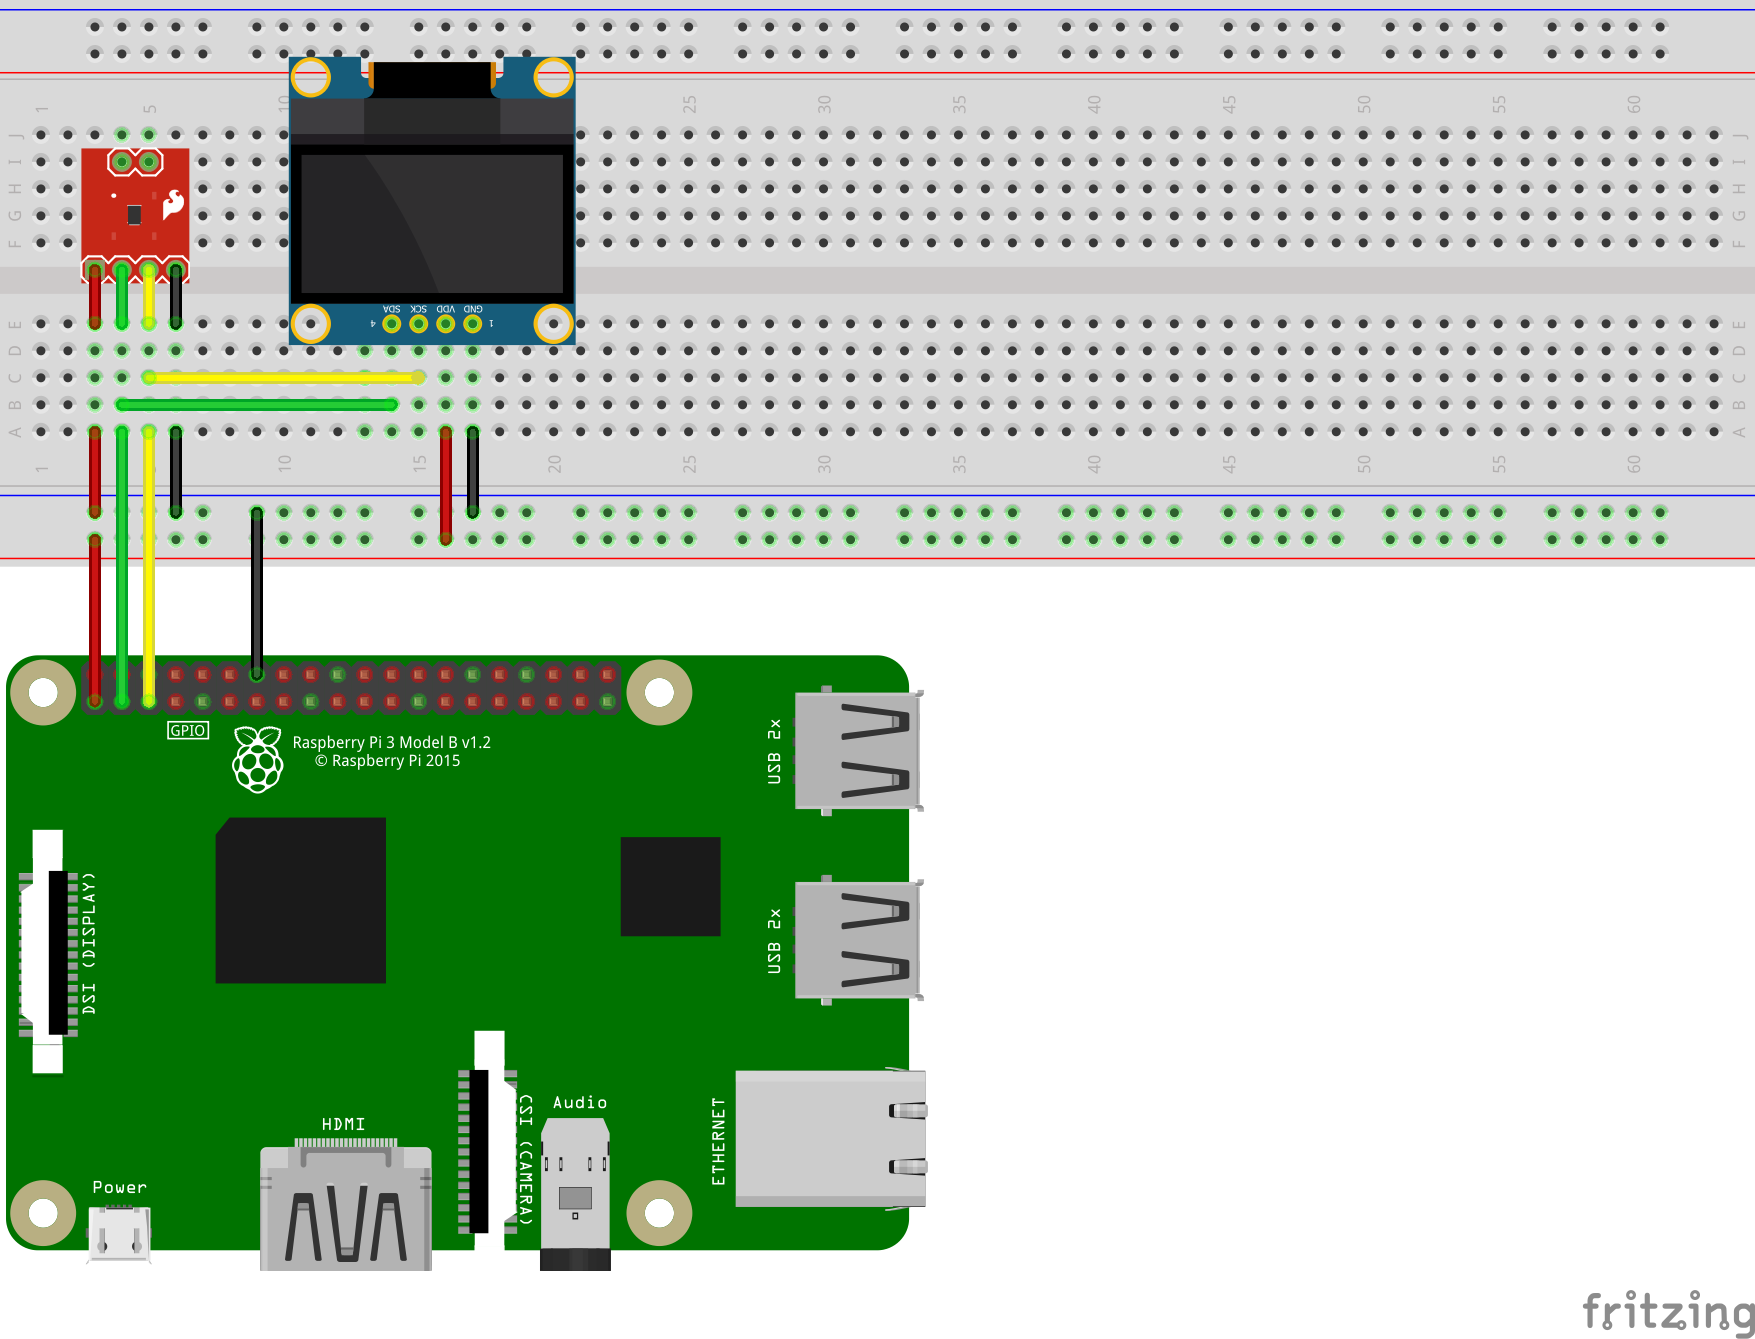
\includegraphics[width=.8\linewidth]{circuit-diagram.png}
	\caption{Circuit diagram for this project}\label{fig:fig1}
\end{figure}

\section{I2C-bus Interface}
I2C (Inter-Integrated Circuit) is a widely used serial communication protocol designed for efficient data transfer between electronic devices. It was developed by Philips (now NXP Semiconductors) and is now an industry standard~\cite{noauthor_i2c-bus_2021}
. The I2C protocol utilizes a master-slave architecture, where a master device initiates communication and controls the data flow, while the slave devices respond to the master's requests. Communication occurs over two lines: a clock line (SCL) and a data line (SDA). The clock line synchronizes the data transfer, while the data line carries the actual information. The I2C protocol supports multiple devices connected to the same bus, each identified by a unique address~\cite{valdez_understanding_2015}
. This allows for easy integration of various components such as sensors, memory chips, and displays into a system. With its simplicity, versatility, and wide support across different microcontrollers and peripherals, I2C has become a popular choice for interconnecting devices in applications ranging from consumer electronics to industrial systems.

Fig.~\ref{fig:fig2} represent a complete data transfer from one device to another~\cite{noauthor_i2c-bus_2021}
. All of I2C components should send data according to the mentioned interface. The I2C-bus is for bi-directional, two-line communication between different ICs or modules. The two lines are a serial data line (SDA) and a serial clock line (SCL). Both lines must be connected to a positive supply via a pull-up resistor. Data transfer may be initiated only when the bus is not busy. Therefore, there are several steps must be followed to avoid concurrent of data among the devices. These process algorithm can be represented as followings~\cite{mankar2014review}
:
\begin{enumerate}
	\item Master Issue START conditions
	\item Slave device get ready
	\item Mater sends the ADDRESS of the device along with access whether read or write
	\item All ICs compare the address with its own
	\item If it does not match, it waits for stop bit
	\item If it matches, it will send an ACK signal
	\item Master receives the ACK signal and start transmitting and receiving data 
	\item Master issue STOP condition
\end{enumerate}

\begin{figure}
	\centering
	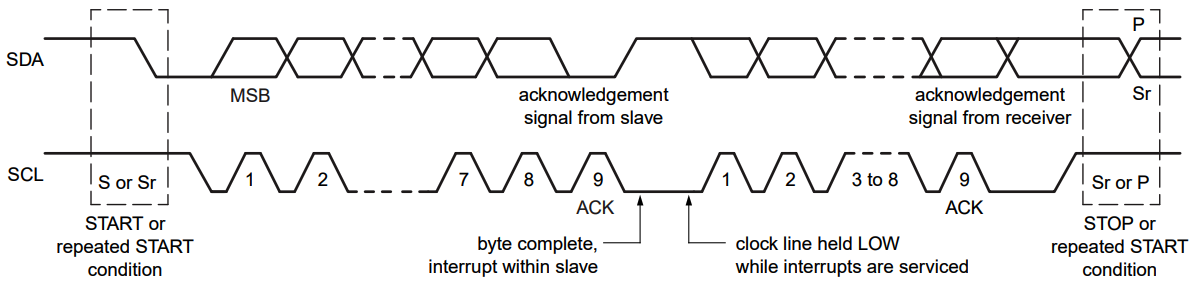
\includegraphics[width=.8\linewidth]{I2CInterface.png}
	\caption{I2C Data Signal with Clock Signal}\label{fig:fig2}
\end{figure}

\section{TMP102}
The TMP102 is a popular digital temperature sensor widely used in various applications. Developed by Texas Instruments, the TMP102 offers high accuracy and low power consumption, making it suitable for both battery-powered devices and industrial systems. This sensor operates over a wide temperature range, typically from -40°C to 120°C, with a resolution of 0.0625°C. It communicates with the raspberry pi through an I2C interface, allowing for easy integration into existing systems. With its compact size and straightforward operation, the TMP102 has become a reliable choice for temperature monitoring in a diverse range of applications, including automotive, consumer electronics, and environmental monitoring systems~\cite{TMP102_datasheet}
.

The data read from the sensor is in binary and therefore must be converted beforehand to be used as degree °C. Followings are the method to convert hex to degree celsius.

\begin{enumerate}
	\item Convert the 12-bit, left-justified binary temperature result, with the MSB = 0 to denote a positive sign, to a decimal number.
	\item Multiply the decimal number by the resolution to obtain the positive temperature.
	\item Example: 0011 0010 0000 = 320h = 800 × (0.0625°C / LSB) = 50°C
\end{enumerate}

\section{SH1107}
The SH1107 is a popular OLED (Organic Light-Emitting Diode) display controller designed for small-size displays. 
Developed by Solomon Systech Limited, the SH1107 offers a compact and efficient solution for driving monochrome OLED panels. 
With its built-in display RAM, the SH1107 enables fast and seamless rendering of graphics and text on the OLED screen. 
The controller communicates with a microcontroller or other host device through an I2C or SPI interface, providing flexibility in system integration. 
The SH1107 also incorporates advanced features such as screen scrolling, contrast control, and a built-in charge pump for generating the required OLED supply voltage. 
Due to its compact size, low power consumption, and versatile capabilities, the SH1107 has gained popularity in various applications, including wearable devices, portable gadgets, and small-scale IoT (Internet of Things) projects. \cite{SH1107_datasheet}

SH1107 differentiate whether the bytes received from Master is data or commands. When the D/Csharp pin is low, the data sent is interpreted as a command. When it is high, the data sent is treated as display data. These followings steps can be taken to configure and write data into SH1107:

\subsection{Initialization}
To initialize the SH1107 controller, specific initialization commands are sent. These commands typically include display configuration settings such as display resolution, multiplex ratio, display offset, and display start line. Additionally, you may need to set the segment remap and common output scan direction to configure the display orientation.

\subsection{Display Control}
The SH1107 offers commands to control the display behavior. These commands include turning the display on or off, setting the display contrast, and inverting the display colors. You can use these commands to adjust the appearance and visibility of the content on the OLED screen.

\subsection{Memory Addressing}
The SH1107 has a display memory that stores the pixel data for the OLED panel. The controller provides commands to set the memory addressing mode. This allows you to choose the addressing mode that suits your specific application requirements, such as horizontal or vertical addressing.

\subsection{Data Writing}
To draw graphics and write text on the display, you need to send the pixel data to the SH1107 controller. The pixel data is typically sent in a sequential manner, following the configured addressing mode. By providing the appropriate pixel data to the controller, you can control the appearance of the content displayed on the OLED screen.


\chapter{Software}
This project consist mostly of software and experimenting with different configuration to produce the best result. This chapter will enlighten the implementation and also the usage of the driver in the API section.

\section{Quick Setup}
The whole project is available at \url{https://mygit.th-deg.de/nb20429/linux-kernel-driver}. User who has access to the git repository can clone the project or download the repository on the website provided to test the drivers. These are the steps to try the drivers.

\begin{enumerate}
	\item Download or clone the drivers. To download the driver, go to the github repository page and click download button. To clone refer to following webpage \url{https://docs.gitlab.com/ee/gitlab-basics/start-using-git.html#clone-a-repository}
	\item Enter the Code folder and open a terminal. Run following command below to clean and rebuild the drivers including inserting module into kernel.
	\item Run the app to see the temperature displayed on SH1107 using the command below.
\end{enumerate}

\begin{verbatim}
bash driver.sh 0
bash driver.sh 1
./app
\end{verbatim}

\section{Implementation}
This section will explain clearly how each of the driver is implemented. The driver file is written in C as both linux and windows are written in C making C as native language to program a driver. These drivers are then compiled into modules using a tool chain called GNU Compiler Collection (gcc) \url{http://gcc.gnu.org/}. GNU also provide assembler, linker, library and object manipulation tools \cite{barry_chapter_2012}.\\

A module must comprise with an Initialization and Cleanup functions \cite{rubini_linux_2001} which can be implemented on Linux using following these lines of codes:

\begin{verbatim}
module_init(my_init)
module_exit(my_cleanup)
\end{verbatim}

\verb'my_init' and \verb'my_clenup' are any functions you want amodule to run when it is inserted and remove respectively. At the end of each driver file, there must be these lines of codes to give the description to the module:

\begin{lstlisting}[language=C]
MODULE_LICENSE("GPL");
MODULE_AUTHOR("Your Name");
MODULE_DESCRIPTION("GPIO Driver");
MODULE_VERSION("1.0");
\end{lstlisting}

with above mentioned characteristics, one should be able to create the driver. Next subsections will show how each of the drivers are implemented.

\subsection{I2C Driver}
This paper will not discuss the whole codes but the algorithm and data structure of the drivers. It is important to note that the devices use I2C for interfacing communication with Raspberry Pi and therefore will need to use the Linux I2C library. These is stated in the header of every driver.\\
Each module has a common file operations structure as followings~\cite{noauthor_character_nodate}:

\begin{lstlisting}
static const struct file_operations fops =
    {
        .owner = THIS_MODULE,
        .open = dev_open,
        .release = dev_release,
        .read = dev_read,
        .write = dev_write
	};
\end{lstlisting}

This means every driver has specific function for read and write. Furthermore several I2C variables need to be configured as followings in every driver~\cite{noauthor_character_nodate}:

\begin{lstlisting}

static struct i2c_adapter *temp_i2c_adapter = NULL;
static struct i2c_client *temp_i2c_client = NULL;
static const struct i2c_device_id device_id[] = {{SLAVE_DEVICE_NAME, 0},{}};
static struct i2c_driver temp_driver = {.driver = {.name = SLAVE_DEVICE_NAME, .owner = THIS_MODULE}};
static struct i2c_board_info i2c_board_info = {I2C_BOARD_INFO(SLAVE_DEVICE_NAME, SLAVE_ADDRESS)};

\end{lstlisting}

\subsection{Initialization and Cleanup}
The source code for TMP102 and SH1107 driver is in file \verb'temp_driver.c' and \verb'display_driver.c' respectively. As a character device there are necessary steps need to be followed to properly initialize it.

\begin{enumerate}
	\item Allocate character device region.
	\item Initialize character device with file operations mentioned above.
	\item Register device with its number.
	\item Create a class in \verb'/sys/class'
	\item Populate \verb'/sys/sysfs' with device info
\end{enumerate}

After character device has properly configured, I2C communication also must be configured. The steps are stated below.

\begin{enumerate}
	\item Assign I2C adapters with an adapter at available I2C bus
	\item Assign I2C client as new I2C client device
	\item Add I2C driver to the susystem
	\item Release asscociated memory of adapter
\end{enumerate}

After the module removed, it is important that the memory allocation for the character device is carefully cleaned and unregistered. This is to avoid any concurrency of memory for future use. The following steps are necessary in \verb'dev_exit' function.

\begin{enumerate}
	\item Unregister I2C device client
	\item Delete driver from the subsystem
	\item Destroy Character device
	\item Destroy Class associated with the device
	\item Delete the character device
	\item Unregister allocated character device region
\end{enumerate}

\section{TMP102}
TMP102 is an Input device which means that the read function must be configured for the device. The read function retrieves temperature data from the TMP102 sensor. It uses I2C communication to read the temperature bytes from the sensor. The received bytes are combined to form a 16-bit integer value representing the temperature. The integer and decimal parts of the temperature are calculated and formatted as a string. The formatted string is then copied to the user space buffer. Finally, the function returns the number of bytes successfully copied.

\section{SH1107}
SH1107 has more complicated implementation compare to TMP102 as it has multiple configuration and special commands before some text can be written on it. Its Write function receives parameters including the file pointer, a buffer containing the data to be written, the number of bytes to write, and the current file offset.

Within the function, there is a maximum length set for the data, which is initially set to 30 bytes but may be adjusted depending on the value of count. The function then attempts to copy the data from the user space buffer into a local buffer. The number of bytes not copied is checked to determine if the copy was successful. \\ Afterward, the last element of data buf is set to null character to ensure it is a valid string. The function then calls the SH1107 String function to display the string on the SH1107 OLED display. \\
Finally, the function returns the number of bytes written to indicate the success of the operation or any error that may have occurred.

There are unique function associated with SH1107 that has been implemented so that it is able to write text on the display comfortably. These functions will explain in next subsections.

\subsection{SH1107 DisplayInit}
This function initializes the SH1107 OLED display. It sends a series of commands via I2C communication to configure the display settings such as:

\begin{enumerate}
	\item 0xAE: turning it off 
	\item 0xA0: setting the segment re-map and common output scan direction 
	\item 0xC0: setting the display mode to normal
	\item 0xA6: setting the memory addressing mode
	\item 0xAF: finally turning on the display
\end{enumerate}

Additional commands can be read from SH1107 Datasheet~\cite{SH1107_datasheet}

\subsection{SH1107 Fill}
This function fills the entire display with a specific data value. It uses nested loops to iterate over each page and column of the display and sends the data value to each pixel using the SH1107 Write function.

\subsection{SH1107 Write}
This function is responsible for sending commands or data to the SH1107 display via I2C communication. It takes two parameters: \verb'is_cmd' indicates whether the data is a command or display data, and data is the actual command or data value. The function constructs a two-byte buffer with the appropriate command data prefix and then calls the I2C Write function to send the buffer over I2C.
This function will call \verb|I2C_Write()| function which is to send data using I2C protocol. The drawing algorithm is as following.

\begin{enumerate}
	\item The data sent are written in hexadecimal in a char array with a size of 2
	\item The first data byte is intepreted whether it is a command or ram data.  When the byte is equal to 0x40, the inputs at D7 - D0 are interpreted as data and be written to display RAM.
	\item When the byte is equal to 0x00, the inputs at D7 - D0 are interpreted as command, they will
	be decoded and be written to the corresponding command registers.
	\item The second byte are the data or a value that should be written.
	\item The Display Data RAM is a bit mapped static RAM holding the bit pattern to be displayed. The size of the RAM is 128 X 128 bits.
	For mechanical flexibility, re-mapping on segment and the direction of common outputs can be selected by software.
	\item This driver used the page address circuit. The page address must be specified first before writing the data.
	\item The next column is automatically adressed with each display data read/write command in vertical addressing mode.
	\item As example a to write as example in \ref{fig:fig1}, The first byte for ram data should be 0xFF indicating \verb|1111 1111|.
	\item The next byte should be  10001000 an so on.
\end{enumerate}

\begin{figure}
	\centering
	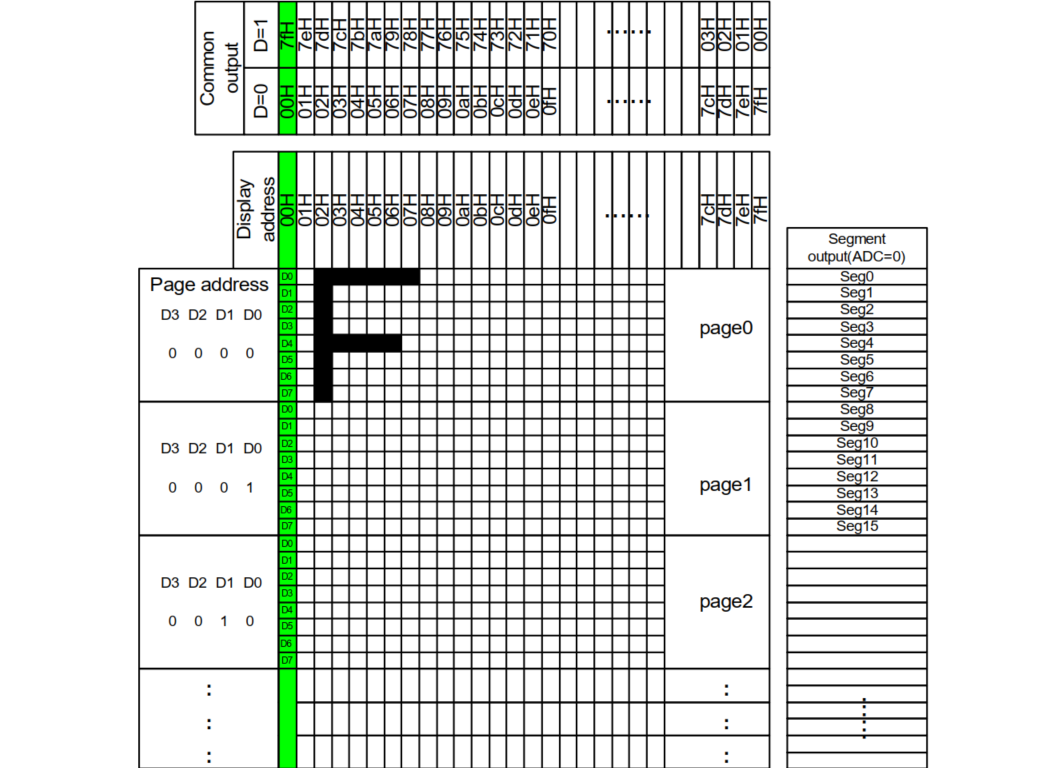
\includegraphics[width=.8\linewidth]{sh1107ram.png}
	\caption{letter ``F'' is written on the ram display}\label{fig:fig1}
\end{figure}

\subsection{SH1107 SetCursor}
This function sets the cursor position on the display. It takes two parameters: lineNo specifies the line number of the display, and cursorPos specifies the cursor position. The function sends the necessary commands to set the page and column addresses using the SH1107 Write function.

\subsection{SH1107 String}
This function displays a string of characters on the SH1107 display. It takes a pointer to a null-terminated string as input. The function iterates over each character in the string and calls the SH1107 PrintChar function to display each character.

\subsection{SH1107 PrintChar}
This function displays a single character on the SH1107 display. It takes a character as input and converts it to the corresponding index in the font table SH1107 font. The function then retrieves the font data for the character and sends it to the display using the SH1107 Write function. It also handles line breaks and backspace characters to manage the cursor position and line wrapping.

\subsection{SH1107 ReturnToFirstSegment}
This function returns the cursor to the beginning of the current line (page) on the display. It fills the remaining segment with zero values using the SH1107 Write function to clear any remaining display data.

\subsection{SH1107 GoToNextLine}
This function moves the cursor to the beginning of the next line on the display. It increments the line number and wraps it around if it exceeds the maximum line value. It then calls SH1107 ReturnToFirstSegment to clear the segment before displaying new data.
\chapter{Usage}
The driver usage example can be found in \verb'i2c_app.c'. This app will display a text ``TEMPERATURE: '' and the temperature in celsius. A library \verb'sys\ioctl' must be included first to use the modules. Each module then must be open first to allow access of using the drivers. After using the module it is advised to close the module using its file descriptor fd.

\section{TMP102}
You can only read data from TMP102 which will return the temperature measured. This can be achieved using following code:

\begin{lstlisting}
read(fd, buf, 100);
\end{lstlisting}

The variable buf must be a string or precisely an array of char. The variable fd is the file descriptor for TMP102 which is \verb'/dev/temp_device'. The int variable 100 indicate the size of char. The string of temperature from the module will be written on the buf.

\section{SH1107}
SH1107 is meant to be an output device, where an app can write data on it, thus producing a text. This can be achieved using following code:

\begin{lstlisting}
strcpy(buf, "\nTEMPERATURE :10.00 ~C");
write(fd, buf, strlen(buf) + 1);
\end{lstlisting}

The array of char buf must be occupied with string first which is by using C library strcpy. To see the font and character capable written by this driver, look at the file \verb'font.h'. In addition to these font there is some unique escape character implemented by this driver such as:

\begin{itemize}
\item \verb'\n' is to go to the next line
\item \verb'\b' is to remove the last character
\end{itemize}
\chapter{Conclusion}
In conclusion, the combination of the TMP102 temperature sensor and SH1107 OLED display offers a powerful solution for temperature monitoring applications. The TMP102 driver provides precise temperature readings with configurable resolution, enabling accurate measurements in various environments. By integrating the SH1107 driver with the TMP102 driver, real-time temperature data can be conveniently displayed on the SH1107 OLED screen.

The TMP102 sensor reliably captures temperature information, while the SH1107 display driver simplifies the process of visualizing the data. With functions for initializing the display, setting the cursor position, and displaying strings, the SH1107 driver allows the temperature readings to be presented in a clear and user-friendly manner on the OLED screen. The ability to accommodate multiple lines of text ensures that the temperature values can be displayed alongside relevant labels or additional information.

By leveraging the capabilities of both drivers, users can create temperature monitoring systems that provide accurate readings and real-time visualization. Whether it's for industrial processes, environmental monitoring, or personal projects, the TMP102 and SH1107 drivers offer a seamless integration that enhances the user experience and facilitates the interpretation of temperature data.

Overall, the TMP102 and SH1107 drivers provide a robust and versatile solution for temperature monitoring. The combined functionality of these drivers enables users to easily display temperature readings from the TMP102 sensor on the SH1107 OLED display, opening up possibilities for a wide range of temperature-based applications.

\bibliographystyle{IEEEtran}
\bibliography{references}
\end{document}
